\section{Streaming-vLLM for Real-Time and Scalable Gameplay}
\label{sec:streaming_vllm}

Real-time gameplay introduces timing constraints that are absent when evaluation pauses the game during inference. The results in Sec.~\ref{sec:exp_cpt_scaling} show that a policy can perform well in a paused game but degrade sharply when the game state changes before its actions arrive. This temporal mismatch also affects online policy optimization: delayed actions change subsequent states and the verified feedback in collected trajectories. At the same time, long-horizon training requires many independent environments to advance concurrently. Practical gameplay and efficient online rollout collection therefore require low-latency serving that preserves state across turns.

We develop \textbf{Streaming-vLLM} as a common execution backend for training, evaluation, and deployment. The backend retains KV states across turns under memory compaction and reduces model execution cost. It also verifies structural tokens proposed by a fast finite-state machine (FSM) and streams verified action blocks before the full packet is complete. The model-facing interface is shared across Qwen3-VL~\cite{qwen3} and Qwen3.5~\cite{qwen35}, including dense and mixture-of-experts (MoE) backbones. Architecture-specific kernels and schedules support each backbone while preserving the same observation–action protocol. Appendix \ref{app:streaming_details} reports representative Dense and MoE serving configurations on Ampere (NVIDIA A800) and Hopper (NVIDIA H200).

\begin{figure*}[!htbp]
    \centering
    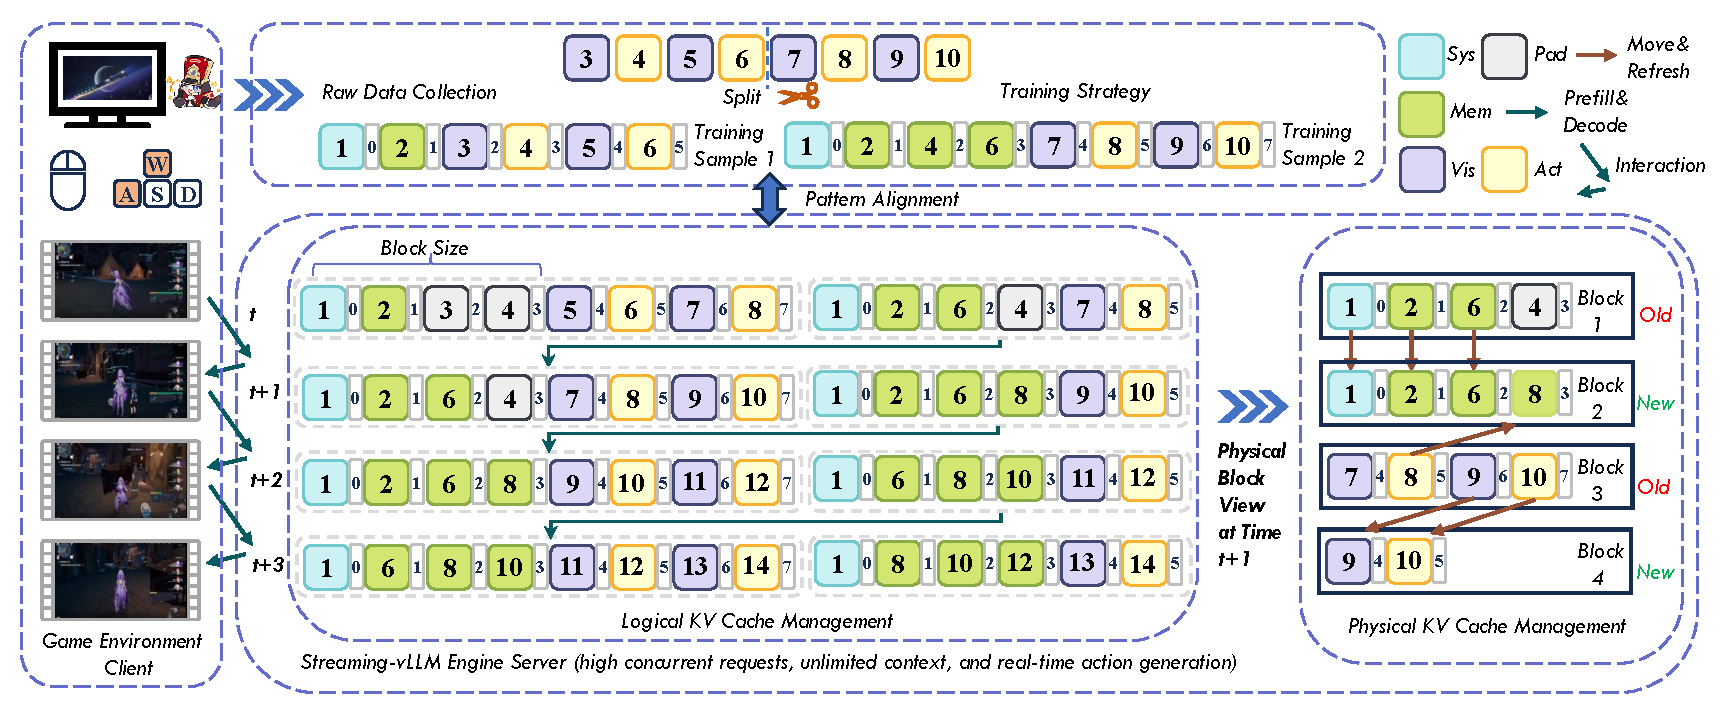
\includegraphics[width=0.89\linewidth]{figs/streaming_vllm.pdf}
    \caption{\textbf{Streaming-vLLM for persistent multi-environment inference.} Each game client maintains separate short-term history, long-term memory, and logical KV-cache state. Two cache forms coexist. Full-Attention layers keep a \emph{growing} paged KV cache: blocks are allocated and reused on demand, and released when context is compacted. In hybrid backbones, gated delta network (GDN) layers instead hold \emph{fixed-size} linear recurrent and convolution states (\texttt{ssm\_state}, \texttt{conv\_state}) whose footprint is independent of sequence length and which are carried across compaction in place. Paged allocation and memory-aware KV-cache reuse avoid repeated context processing, while incremental rotary position embedding (RoPE) refresh corrects retained keys after compaction. The runtime combines architecture-aware execution, BF16-verified FSM speculation, and early action dispatch to serve concurrent real-time interactions.}
    \label{fig:streaming_vllm}
\end{figure*}

\subsection{Memory-Compacted Streaming Context}
\label{sec:streaming_context}

At each interaction step, the model consumes the control specification, task instruction, long-term memory, and recent observation-action history $(\mathcal B,I,\mathcal M_t,\mathcal H_t)$. Re-encoding the visual and textual history at every turn would repeat the same prefill work. As shown in Figure~\ref{fig:streaming_vllm}, Streaming-vLLM instead preserves KV states of retained context and computes new states only for newly appended tokens, following stateful streaming inference~\cite{xiao2024streamingllm,xu2026streamingvlm}. A short-term queue holds recent complete interaction rounds, while a long-term queue stores generated memory summaries. At a compaction boundary, the policy summarizes history before eviction. The discarded rounds release their KV pages, and recent rounds retain cached states. Each environment keeps its own logical-to-physical block table over the paged allocator~\cite{kwon2023pagedattention}, allowing requests with different history lengths to coexist.

Compaction also changes the logical token positions of retained states. We update the rotary phase of the corresponding cached keys using the positional shift, without recomputing their projections or modifying the value cache; in hybrid backbones, gated-delta-network (GDN) layers carry no rotary phase and instead retain their fixed-size linear recurrent and convolution states in place across eviction boundaries. The retained cache preserves state across turns, so it need not be numerically equivalent to a full re-encoding of the shortened context. The precise RoPE refresh and its scope are detailed in Appendix~\ref{app:rope_refresh}. The same bounded history and persistent summaries are used in SFT and to link TA-GRPO trajectory segments.

\subsection{Architecture-Aware Execution Across Backbones}
\label{sec:streaming_backend}

Frequent short requests incur costs beyond prefill, including decoder launches, inter-device communication, and architecture-specific operations. Streaming-vLLM separates a common serving interface from specialized execution paths. Dense and MoE variants share action serialization, context compaction, and client scheduling, while the compute backend accommodates their respective attention, expert, and recurrent or gated-delta-network operations. We combine operator fusion, tensor-parallel execution, communication overlap, and CUDA Graph replay to reduce serial overhead. We apply tensor parallelism selectively. It can reduce decoder compute time, but communication and synchronization may outweigh the savings for the smaller ViT workload. The measured tradeoff is analyzed in Table~\ref{tab:streaming_vllm_ablation}. Across Ampere and Hopper GPUs, decode and speculative verification are each implemented as an all-layer megakernel that combines fine-grained L2 prefetching, in-place cross-rank reduction and normalization, and a fused sampling and state-machine tail to minimize CPU and synchronization overhead. For vision encoding and context prefill, persistent kernels overlap tile-level communication with computation and fold cross-rank reduction and normalization into the GEMM epilogue. Finally, W8A8 quantization yields only modest end-to-end gains and is applied selectively: ViT remains in BF16 to avoid low-precision representation instability, prefill quantizes only large QKV and MoE expert projections to prevent router flips and GDN state drift across short single-frame extensions, and low-batch decode is latency- and barrier-bound rather than compute-bound.

We assess portability across model families and hardware configurations. Our supported model set spans Qwen3-VL~\cite{qwen3} dense 2B, 4B, 8B, and 32B and MoE 30B-A3B, together with Qwen3.5~\cite{qwen35} dense 0.8B, 2B, 9B, and 27B and MoE 35B-A3B. Our experiments and analysis cover representative Qwen3-VL Dense and Qwen3.5 MoE workloads across datacenter Ampere and Hopper GPUs. The appendix compares numerical precision and tensor-parallel settings on each GPU. Beyond these datacenter architectures, because the kernel pipelines and tile schedules are parameterized by SM count, register budget, shared-memory ceiling, and L2 capacity at runtime, the same execution paths also extend to Ada Lovelace and Blackwell GPUs. Although these platforms face much tighter inter-GPU communication constraints without NVLink peer-to-peer interconnect, a custom communication layer encapsulates zero-copy host-mapped shared memory, system-scope lock-free release/acquire primitives, and payload-adaptive collective schedules behind an unchanged model-facing interface. These extensions are included for architectural portability and compatibility rather than benchmark comparison.

\subsection{Verified FSM Decoding and Streaming Actions}
\label{sec:streaming_action}

After execution overhead is reduced, autoregressive generation remains sequential. A fast finite-state-machine (FSM) drafter proposes predictable structural tokens in the reasoning–action output. The FSM tracks \texttt{<think>}, \texttt{</think>}, \texttt{<|action\_start|>}, and \texttt{<|action\_end|>} boundaries. It proposes closing an empty reasoning span or starting an action packet after reasoning ends. Within the action, it drafts whitespace after mouse-coordinate numbers, the separator following the Z coordinate, and predictable delimiters and empty-key patterns across the six keyboard-mouse groups. \textbf{Mouse-coordinate values remain model-generated.} During generation, the FSM enforces constrained sampling over valid transitions via state-dependent vocabulary bitmasks at every decoding and verification position, while simultaneously packing candidate continuations from the next grammar states into a draft tree that the target model verifies through a single shared-prefix pass~\cite{leviathan2023fast,zheng2024sglang,miao2024specinfer,cai2024medusa,li2024eagle}, committing only accepted prefixes. The policy retains control over action selection, while verification reduces the number of sequential decoding iterations. See Appendix~\ref{app:speculative_sampling} for more details.

Streaming-vLLM also reduces the time to the first executable action. Once the mouse fields and first verified key block are ready, the server sends that prefix to the client while the remaining blocks continue decoding. The client executes the six blocks in order, maintaining key press-hold-release semantics. Action execution can therefore begin while the remaining blocks are still being generated. The theoretical block-generation rate reported in the system ablation and the nominal 30~Hz client control protocol are distinct measurements, as clarified in Appendix~\ref{app:streaming_latency}.

\subsection{Concurrent Serving for Online Rollouts}
\label{sec:streaming_serving}

Real-time rollouts require scheduling that accounts for both action deadlines and throughput. Each active environment is assigned an isolated resident state slot that holds its short-term history, long-term memory, and model states, avoiding context rebuilds when environments alternate turns. The runtime time-division multiplexes incoming frames' vision encoding and context extension across slots over a shared workspace, and then performs batched token generation and verification across all ready environments. Within each slot, paged KV caches and linear recurrent (GDN) states follow different update rules during scheduling: KV caches are position-indexed, so speculative tokens write directly to trailing slots and rejected suffixes are simply overwritten on the next step, whereas fixed-size recurrent states update in place and are committed only for the accepted prefix after verification. This balances aggregate throughput against the progress rate of each active environment. Real-time evaluation and TA-GRPO training share the same serving path, so training rollouts are collected under the same execution protocol while the game continues to advance.

Stateful cache reuse reduces the cost of long contexts, architecture-specific backends support different models and GPUs, and verified FSM drafting reduces action-generation cost. Combined with early action dispatch, these components enable responsive, high-frequency control and parallel RL rollouts linked by memory summaries. Section~\ref{sec:exp_streaming} reports latency and closed-loop evaluations, and Appendix~\ref{app:streaming_latency} provides representative GPU, precision, and parallelism settings.
